\begin{frame}
	\frametitle{\problemtitle}
	\begin{block}{Problem}
		Given at most $2\cdot 10^5$ frogs with integral positions, and a list of
		at most $10^6$ frog-IDs (events).
		For each ID in the list, move the corresponding frog to the next free
		position.
	\end{block}
	\begin{center}
		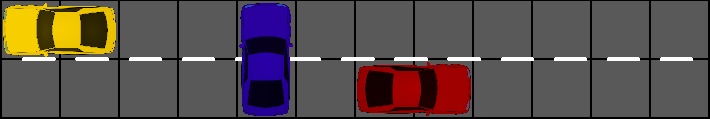
\includegraphics[width=0.33\textwidth]{sample}
	\end{center}
	\pause
	\begin{block}{Solution}
		\alt<6->{
			\begin{itemize}
				\item<6-> Maintain the current positions of each frog and an ordered set $S$ of currently free positions.
				\item<7-> Now the events can be simulated quickly. For a jump of frog $i$, currently at position $p$:
					\begin{itemize}
						\item find $\min\{p'\in S : p < p'\}$ in $\mathcal{O}(\log{|S|})$ using operations from the standard library.
						\item update $S$ and the position of frog $i$
					\end{itemize}
				\item<8-> Total time complexity: $\mathcal{O}(n \log{|S|})$
			\end{itemize}
		} {
			\begin{itemize}
				\item Store for each position whether it is occupied or not in an array.
					Only positions up to $1.2\cdot 10^6$ are relevant.
					\pause
				\item Now, simulate the events: For a jump of frog $i$,
					currently at position $p$, scan the ``occupied''-array
					starting at $p$ and seek the next free position.
					\pause
				\item Time complexity? \pause $\mathcal{O}(n^2)$ This is too
					slow (unless very very very optimised\dots)
			\end{itemize}
		}
	\end{block}
	\pause
\end{frame}
